\documentclass[uct_visualisation_thesis.tex]{subfiles}

\section{Instalacja}
\subsection{Wymagania sprzętowe}
W celu wykorzystania możliwości, które daje prezentowany system, należy uruchomić go na komputerze, który spełnia wymienione poniżej wymagania sprzętowe.

\begin{enumerate}
	\item Procesor: Intel Core i5-3470 3.2 GHz / AMD FX-8350 4 GHz.
	\item Pamięć RAM: 8 GB.
	\item Karta graficzna: Nvidia GTX 660 2GB / AMD HD 7870 2 GB.
	\item Miejsce na dysku twardym: 150 MB.
	\item System operacyjny: Windows 10 / Ubuntu 16.04.
\end{enumerate}

\subsection{Instrukcja instalacji}
W celu zainstalowania aplikacji na dysku lokalnym należy rozpakować jedno z dostarczonych archiwum. Prezentowany system został zbudowany w formie aplikacji przenośnej, więc wszystkie komponenty potrzebne do uruchomienia aplikacji są dostarczone razem z nią. W zależności od systemu operacyjnego urządzenia, należy wybrać odpowiednio:

\begin{enumerate}
	\item dla urządzeń z systemem Windows - \textit{UCTVisualisation-portable.zip},
	\item dla urządzeń z systemem Linux - \textit{UCTVisualisation-portable.tar}.
\end{enumerate}


\subsection{Instrukcja uruchamiania}
Zainstalowana aplikacja znajduje się w rozpakowanym katalogu o nazwie \textit{UCTVisualisation}. Aby uruchomić aplikację uruchomić odpowiedni plik w rozpakowanym katalogu. W zależności od systemu operacyjnego urządzenia, należy wybrać odpowiednio:
\begin{enumerate}
	\item  dla urządzeń z systemem Windows - \textit{UCT Visualisation.exe},
	\item dla urządzeń z systemem Linux - \textit{UCT Visualisation}.
\end{enumerate}


\subsection{Instrukcja uruchamiania na urządzeniach z systemem Linux}
W celu instalacji programu na lokalnym dysku, potrzebne jest uruchomienie pliku \textit{UCTVisualisationSetup.deb}, a następnie kliknięcie przycisku.
Aplikacja o nazwie \textit{UCT Visualisation} znajduje się w katalogu o takiej samej nazwie i domyślnie zostaje zainstalowana pod ścieżką:


\section{Mankala}
\subsection{Wstęp}
Mankala, jako jedna z przykładowych gier modułu \textit{Gry}, jest mniej popularną grą logiczną od szachów, więc postanowiono przedstawić instrukcję rozgrywki.\\

Plansza mankali zawiera dwanaście mniejszych pól i dwa większe, nazywane domami lub bazami. Każdemu z graczy przypisane jest sześć mniejszych pól leżących przed nim i dom po jego prawej stronie. Na początku gry w każdym z pól znajdują się cztery kamienie. Celem obu graczy jest zebranie jak największej liczby kamieni w ich domach. Gra kończy się, gdy wszystkie pola jednego z graczy są puste -- wtedy pozostałe kamienie przydzielane są drugiemu graczowi.

\begin{figure}[h!]
	\centering
	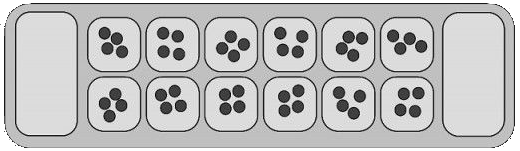
\includegraphics[width=0.6\textwidth]{mancala.png}
	\caption{Plansza mankali}
	\label{rys:mancala}
\end{figure}

\subsection{Ruch gracza}
Ruch gracza polega na wyjęciu wszystkich kamieni z wybranego własnego pola i rozdysponowaniu po jednym do kolejnych pól, omijając dom przeciwnika. Rozdysponowanie jest wykonywane w kierunku odwrotnym do ruchu wskazówek zegara. Ponadto, jeśli ostatni kamień wyląduje we własnym domu -- gracz musi wykonać kolejny ruch. W przeciwnym przypadku -- następuje ruch przeciwnika.

\subsection{Bicie}
Ostatnią zasadą mankali jest bicie. Bicie następuje, jeśli po wykonaniu ruchu, ostatni kamień wyląduje na pustym polu gracza. W takiej sytuacji gracz zabiera wszystkie kamienie z przeciwległego pola planszy. Jeżeli w sąsiednim polu nie ma kamieni, nie dochodzi do ich przejęcia. Tak samo, ruch nie kończy się biciem, jeżeli ostatni kamień wyląduje na pustym polu przeciwnika.